\chapter{0620 Safety Policy}
The M:2:I Lab Space is a multifunction lab and shop space that allows students to work on their projects in a safe environment.  The M:2:I Lab gives students the ability to design, build, test and learn from their projects.  Use of this lab space however is a privilege, and therefore students must follow all rules, policies and procedures or risk temporarily or permanent removal from the lab.

All students using the lab space must have the following trainings complete:

\begin{itemize}
\item EH\&S PPE Training
\item EH\&S Fire Training
\item M:2:I General Lab Training
\end{itemize}

Additional trainings for other tools in the lab may also be required.  Students that do not have these training completed will not be allowed to use the lab space or equipment.  For more information please see the M:2:I Training Manual.

\section{Student Conduct}
Students working in the lab must not work alone.  No student should be in the lab by themselves.  Working alone in the lab is a major safety concern as if something happens to that student, they would have no method to call for help.  

No horseplay is permitted at any time in the lab.  Students should never attempt to startle or surprise any person that is working in the lab.  Students are expected to maintain a professional environment at all times while working in the lab.

\section{Personal Protective Equipment}
While we have worked hard to make the 0620 lab space as safe as possible, hazards are still present in the lab when construction and other tasks are taking place.  Students can reduce their risk of injury by wearing the appropriate safety equipment.  Some \index{PPE} is required while others may be optional but are desired.  Students are ultimately responsible for their own safety.  The policies set forth here are to guide students on what the lab requires students to wear.  Training on safety equipment can be found in the M:2:I Training Manual.

\subsection{Dress Code}
Students working in the M:2:I Lab must follow the following \index{dress code}:

\begin{itemize}
\item No open sole shoes at any time
\item No loose clothing
\item No shorts or skirts
\end{itemize}

Students should expect to dress as though they are working with tools and equipment in the lab at all times.  

\subsection{Safety Glasses}
\index{Safety glasses} must be worn in designated safety glasses areas. Figure \ref{fig:0620_floor_plan} shows the floor plan of the 0620 lab space.  Areas in yellow must have safety glasses worn at all times.  No tools that require safety glasses may be used outside the designated areas.

\begin{figure}[ht]
\centering
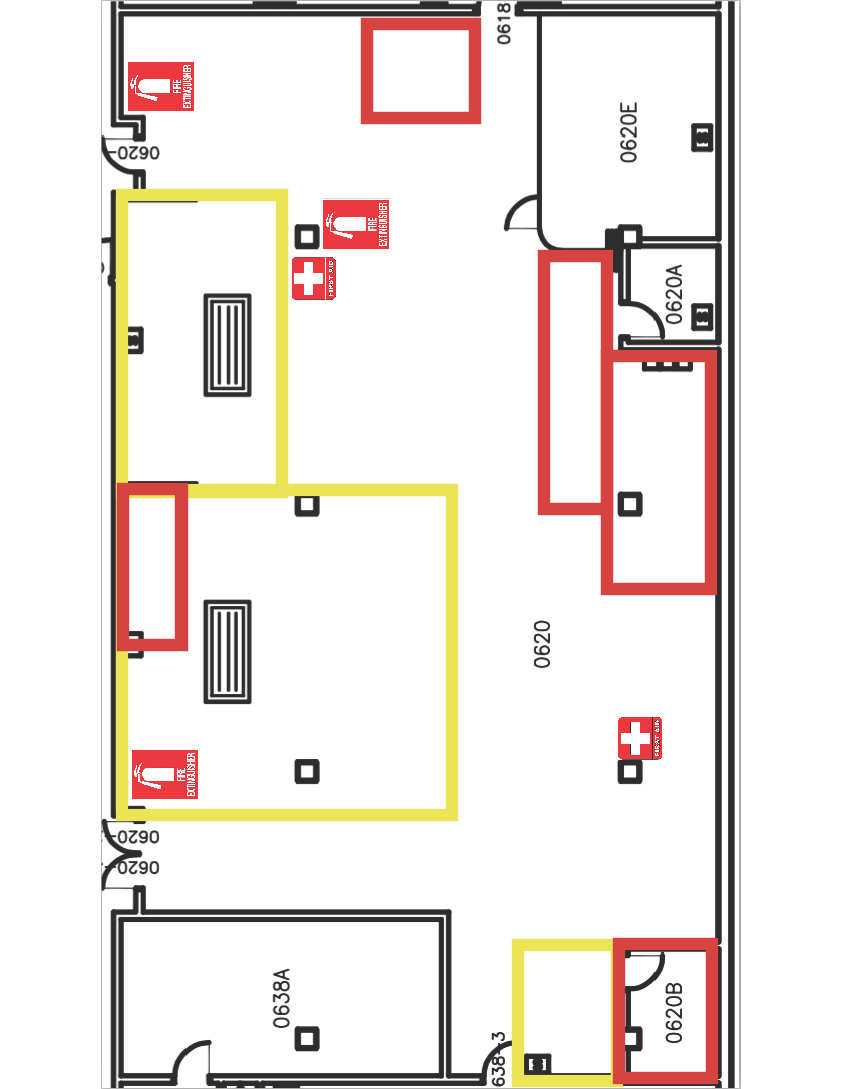
\includegraphics[width=5in]{images/0620_Floor_Plan.png}
\caption{0620 Floor plan with safety glasses and restricted areas marked}
\label{fig:0620_floor_plan}
\end{figure}

Safety glasses must be \index{ANSI Z87.1} approved.  Safety glasses must be marked with a Z87 as the minimum requirement and Z87+ is preferred for use the 0620 lab.  An example of the marking that should be shown is in Figure \ref{fig:ansi}.  Lightly tinted safety glasses may be used but fully tinted safety glasses are not permitted.  Students that wear prescription glasses may use those glasses only if the glasses are also ANSI Z87.1 approved and properly marked.  The appropriate side shields must also be installed and must also meet ANSI Z87.1 approval.

\begin{figure}[ht]
\centering
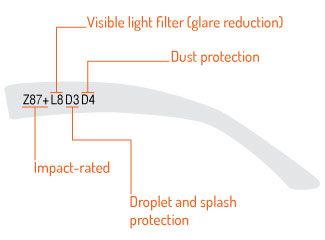
\includegraphics[width=4in]{images/ansi-z871.jpg}
\caption{Safety glasses with proper ANSI marking}
\label{fig:ansi}
\end{figure}

\subsection{Gloves}
The M:2:I Lab space has \index{nitrol gloves} that well suited for working with adhesives, paints and other materials that may cause chemical irritations to the skin.  These gloves  must be worn and the work surface must be protected when working with adhesives, paints or other solvents. Make sure you select the correct glove size for your hand so they are comfortable to use.

Leather or cloth gloves may be used if desired when working with wood or other materials.  However, these are not provided to students.  Use of gloves near \index{power tools} such as the \index{bansaw} or drill may cause a hazard if care is not taken to ensure the gloves do not get caught up in the machine.  For this reason, we leave the use of these gloves to the personal preference of the student using the machine.  Students however should consult either the M:2:I Program Coordinator or other faculty and staff if they have questions on what they should wear.  

\subsection{Masks}
The M:2:I Lab has \index{filtration masks} that are useful for filtering small and large particulates from the air when working.  Masks must be worn when sanding or working with aerosols. The masks that are provided are disposable and may only be used once per session.  Anytime that masks are required, safety glasses are also required to be worn.
